% !TeX encoding = UTF-8

\documentclass{LTHtwocol} % Use this when you work on your report.
% \documentclass[final]{LTHtwocol} % Use this for the final version.
                                   % It will remove page numbers and
                                   % markers for overfull boxes.
                                   % There really shouldn't be any of those anyway.

\usepackage[utf8]{inputenc}
\usepackage{amsmath,amssymb,graphicx}
\usepackage{float}
\usepackage{xcolor}
\usepackage{hyperref}
\hypersetup{
	colorlinks,
	linkcolor={red!50!black},
	citecolor={blue!50!black},
	urlcolor={blue!80!black}
}

\usepackage{kantlipsum} % Only for the dummy text. Remove for your own report.

\addbibresource{bibliography.bib}

% Document begins here
\begin{document}
\begin{frontmatter}
\title{Balance Double Inverted Pendulum on Cart} % Title of the project.
                      							 % Note that all reports are in English,
							                     %so that our international students can read them.

\author[cem]{Cem Alpt\"urk}
\author[pukashawar]{Pukashawar Pannu}

\email[cem]{ce5368al-s@student.lu.se}
\email[pukashawar]{pu6218pa-s@student.lu.se}

\begin{abstract}
    The abstract should be a 200--250 word compact description of your project. What was the objective? Which methods did you use? What was the (main) result?
\end{abstract}

\end{frontmatter}

% Stick to the proposed structure below. Add \subsections{} as appropriate.
% This file compiles on the Automatic Control Department system by typing the
% following into the terminal (while in the directory of the file, and with all
% other files belonging to the template untouched):
% > pdflatex template
% > biber template
% The first line compiles the .tex file. The second line generates the
% bibliography. Once this is done, you may need to run the first line 1-2
% additional times, for the system to get all cross references right in the
% produced pdf output.

\section{Introduction}
The goal of this project is to teach an agent to control a double pendulum on a cart to be standing upright, in its equilibrium point, using reinforcement learning.
A double pendulum is a highly chaotic system, where its behavior heavily depends on its initial conditions.
As a result, this system can be very difficult to control. 
Figure \ref{fig:double_pendulum_chaotic} shows a simulation with 4 double pendulums with nearly identical initial conditions.
After some time their behaviors become so different that it becomes nearly impossible to make a prediction about the future.
This illustrates the chaotic behavior of this system.
Our aim is to create an agent that can learn from its own experiences to control the double pendulum, by applying a force on the cart in the horizontal direction, such that it stays upright.
Although this is an academic problem, the results could be applied to any type of learning problem since the agent is unaware of what its working on.
(Possible reference to qlearning)
\begin{figure}[H]
	\centering
	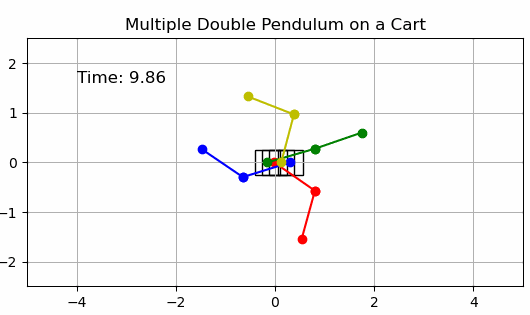
\includegraphics[width=0.7\columnwidth]{figures/Double_Pendulum_Chaotic_2.PNG}
	\label{fig:double_pendulum_chaotic}
	\caption{4 double pendulums simulated with similar initial conditions after $9.86$ seconds, with a difference of $0.02 rad/s$ differences on the inner pendulum angular velocities. All other initial states were equal.} 
\end{figure}
% Here you introduce the project. What is the background? What project do you aim at solve? References to prior work? If the project makes a positive or negative environmental, or other solitary, impact, describe it here. Are there any ethical considerations? You might want to reference relevant literature, e.g. \cite{openclosed2, Hellerstein2004, Yun2015}. A general \LaTeX\ guide is available at \cite{latexwiki}.

\subsection{Reinforcement Learning}
%\kant[1] % This generates the dummy text
The main idea of reinforcement learning is to learn to make decisions based on past experiences. 
In this case this means to train an agent that performs the best action, the force applied in the horizontal direction,  possible given the current states of the system.
For each action taken by the agent, the environment returns a new state and a reward for that action. 
The reward is calculated based on how close the system is to its equilibrium point.
The goal of training the agent is to optimize gained reward for each action taken.

\section{Modeling}
The system consists of a cart that can move in the horizontal direction and two pendulums that are coupled to each other such that there is no collision between any parts.
Since this project is not about modeling the double pendulum, but rather about controlling it, we have borrowed the equations of motion from (ref).
The states of the system are represented by,
\begin{equation}
x  := 
\begin{bmatrix}
y & \dot{y}
\end{bmatrix}
^T , \quad y := 
\begin{bmatrix}
q & \theta_1 & \theta_2
\end{bmatrix}
^T
\end{equation}
%\begin{equation}
%x :=
%\begin{bmatrix}
%q & \theta_1 &  \theta_2 &  \dot{q} &  \dot{\theta_1} & \dot{\theta_2}
%\end{bmatrix}
% ^T
%\end{equation}
\begin{itemize}
\item $q$ is the position of the cart on the horizontal axis.
\item $\theta_1$ is the angle of the inner pendulum with respect to the vertical axis in the clockwise direction.
\item $\theta_2$ is the angle of the outer pendulum with respect to the vertical axis in the clockwise direction.
\item $\dot{q}$ is the velocity of the cart in the horizontal axis.
\item $\dot{\theta_1}$ is the angular velocity of the inner pendulum.
\item $\dot{\theta_2}$ is the angular velocity of the outer pendulum.
\end{itemize}

The system parameters are represented by,
\begin{itemize}
\item $m = 1 [kg]$ is the mass of the cart.
\item $m_1 = 0.1 [kg]$ is the mass of the inner pendulum.
\item $m_2 = 0.1[kg]$ is the mass of the outer pendulum.
\item $l_1 = 1 [m]$ is the length of the inner pendulum.
\item $l_2 = 1[m]$ is the length of the outer pendulum.
\item $g = 9.81 [m/s^2]$ is the gravitational acceleration.
 \end{itemize}

The equations of motions for this system (ref), are adjusted such there is no friction or disturbances. 
The input to the system is a horizontal force that is acting on the cart, represented by $u$ $[N]$.

\begin{equation}
M(y) \ddot{y} = f(y,\dot{y},u)
\end{equation}


\begin{equation}
\resizebox{ \columnwidth}{!} 
{
$
M(y) := 
\begin{bmatrix}
m + m_1 +m_2 & l_1(m_1+m_2)\cos \theta_1 & m_2 l_2 \cos \theta_2 \\
l_1 (m_1 + m_2) \cos \theta_1 & l_1^2(m_1+m_2) & l_1 l_2 m_2 \cos(\theta_1 - \theta_2) \\
l_2 m_2 \cos \theta_2 & l_1 l_2 m_2 \cos (\theta_1 - \theta_2) & l_2^2 m_2
\end{bmatrix}
$
}
\end{equation}

\begin{equation}
\resizebox{ \columnwidth}{!} 
{
$
f(y,\dot{y},u) :=
\begin{bmatrix}
l_1(m_1+m_2) (\dot{\theta_1})^2 \sin \theta_1 + m_2 l_2 (\dot{\theta_2})^2 \sin \theta_2 + u\\
-l_1l_2m_2(\dot{\theta_2})^2 \sin(\theta_1 - \theta_2) + g(m_1 + m_2)l_1 \sin \theta_1 \\
l_1l_2m_2(\dot{\theta_1})^2 \sin (\theta_1 - \theta_2) + g l_2 m_2 \sin \theta_2
\end{bmatrix}
 $
 }
\end{equation}




 

%Here you present the modeling approach and publish your model. If your model has 63434 parameters, you may not wish to print it in detail. The idea is, however, that another group with your background should be able to reproduce your work -- this goes not only for the modeling aspect.
%
%If you use equations, make sure they are all numbered:
%\begin{equation}
%\alpha_a^2 + \beta_b^2 = \gamma_c^2.
%\label{eq:formula}
%\end{equation}
%Equations are parts of the text. If they end a sentence, they should end with a dot. If they end a clause, they should end with a comma. You refer to an equation this like: see \eqref{eq:formula}. Note that all units are written in roman type: $\omega=2\pi$~rad/s, $g = 9.81$~m/s$^2$. See \cite{mathslatexwiki} for a tutorial on typesetting maths.
%
%\subsection{Some Dummy Text}
%\kant[2]

\section{System Design}
Describe the control or learning system you have designed.
Did you build anything? If so, what did you build, and using what production methods. If you built the hardware or were handed it, \emph{a photograph of your gadget is mandatory}. Make sure any figures are referenced from from the text---like this, see Figure~\ref{fig:gadget}---and that they all have a descriptive caption.
\begin{figure}[b]
	\centering
	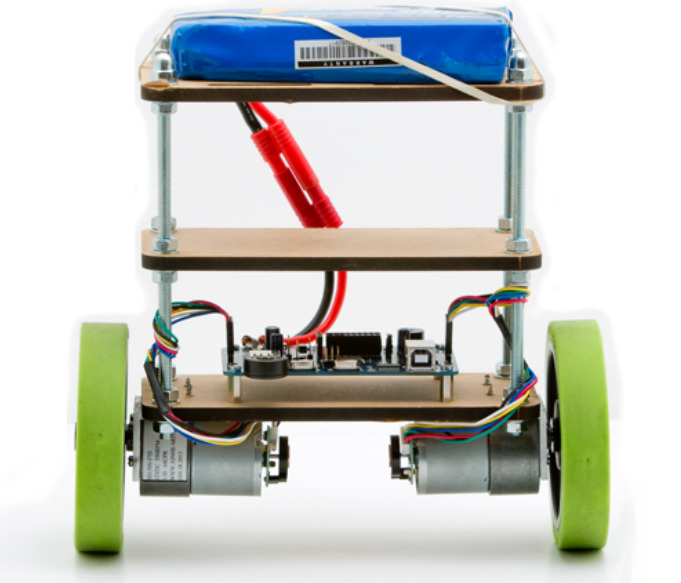
\includegraphics[width=0.7\columnwidth]{balanduino}
	\caption{Example picture of the Balanduino robot. Place all figures at the top \texttt{[t]} (default) or bottom \texttt{[b]} (only if needed).}
	\label{fig:gadget} % Should be placed after the caption!
\end{figure}

\subsection{Some Dummy Text}
\kant[3]

\section{Implementation}
Here you describe how you implemented your learning or control design.

\section{Results}
If you need to use tables, Table~\ref{tab:extable} shows an example of how they can be typeset. For further details, see \cite{tablelatexwiki}.

\begin{table}[t]
	\centering
	\caption{Example table. Note that the caption goes on top. Place all tables at the top \texttt{[t]} (default) or bottom \texttt{[b]} (only if needed) of the page.}
	\label{tab:extable}
	\begin{tabular}{lcrrcrrcrr} % (l)eft, (r)ight and (c)enter indentation
		\toprule
        &
		\multicolumn{2}{c}{IAE [$\cdot 10^3$~s]} & &
		\multicolumn{2}{c}{$\text{var}(\tau^o)$ [s]} & &
		\multicolumn{2}{c}{$\tau^o_{max}$ [s]} \\[1mm]
		$M_C$            &  3     & 10  &~& 3     & 10    &~& 3    & 10 \\
        \midrule
		$C_{\text{orig}}$ & 8.23 & 8.34 &~& 0.695 & 0.745 &~& 5.68 & 6.27 \\
		$C_{\text{fb}}$ & 1.48 & 0.98 &~& 0.030 & 0.021 &~& 1.81 & 1.83 \\
		$C_{\text{ff}}$ & 1.23 & 1.43 &~& 0.026 & 0.034 &~& 1.56 & 1.65\\
        \bottomrule
	\end{tabular}
\end{table}

\subsection{Some Dummy Text}
\kant[4]

\section{Discussion}

Discuss the results and what you learned from the project.


% Prints cited references
\printbibliography


\end{document}
